\section{ EM, Shift-Invariant Models and Deblurring}

\subsection{Shift-Invariant Models}
In this problem we will consider shift-invariant mixtures of multi-variate multinomial distributions.
\\
\\
Consider data that have multiple discrete attributes. ``Discrete'' attributes are attributes that can take only one of a countable set of values.  We will consider discrete attributes of a particular kind -- integers that have not only a natural rank ordering, but also a definite notion of distance. 
\\
\\
Let $(X,Y)$ be the pair of discrete attributes defining any data instance.  
Since both $X$ and $Y$ are discrete, the probability distribution of $(X,Y)$ is a bi-variate multinomial.
\\
\\
We describe $(X,Y)$ as the outcome of generation by the following process:
\\
\\
The process has at its disposal several urns.  Each urn has \textbf{two} sub-urns inside it.  
The first sub-urn represents a bi-variate multinomial:  it contains balls, such that each ball has an $(X_1,Y_1)$ value marked on it.
The second sub-urn represents a uni-variate multinomial -- it contains balls, such that each ball has a $X_2$ value marked on it.

\begin{center}
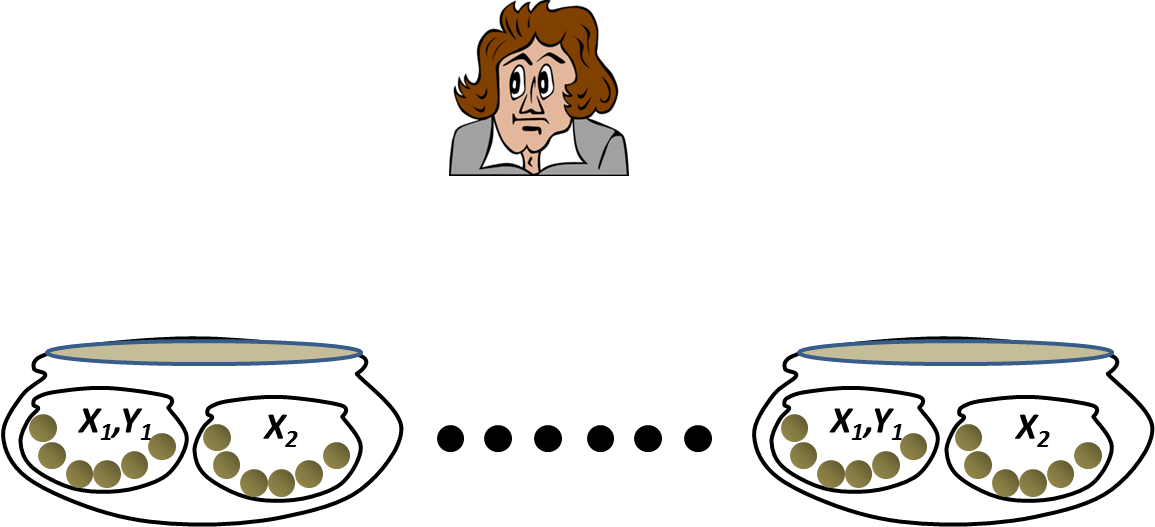
\includegraphics[scale=0.4]{figs/process.png}
\end{center}
In the following explanation we will use the notation $P_x(X)$ to indicate the probability that the \textit{Random Variable} $x$ takes the value $X$.
\\
\\
We represent the content of the larger sub-urn within each urn as $(x_1, y_1)$. The smaller sub-urn generates the random variable $x_2$.
\\
\textbf{Drawing procedure}: At each draw the drawing process performs the following operations.
\begin{itemize}
\item It first randomly selects one of the larger urns according to a probability distribution $P_z(Z)$. Here $Z$ represents the urn selected.
\item Then it selects one ball from each of the sub-urns in the selected urn. The probability of balls in the $(x_1,y_1)$ sub-urn of the $Z^{\text{th}}$ urn is $P_{x_1,y_1|z}(X_1,Y_1|Z)$. The probability of balls in the $(x_2)$ sub-urn of the $Z^{\text{th}}$ urn is $P_{x_2|z}(X_2|Z)$. Drawing from these distributions, the process obtains a $(X_1,Y_1)$ pair from the $(x_1, y_1)$ sub-urn, and $X_2$ from the $x_2$ sub-urn
\item It finally outputs  $(X,Y) =  (X_1 + X_2, Y_1)$.
\end{itemize}
\begin{center}
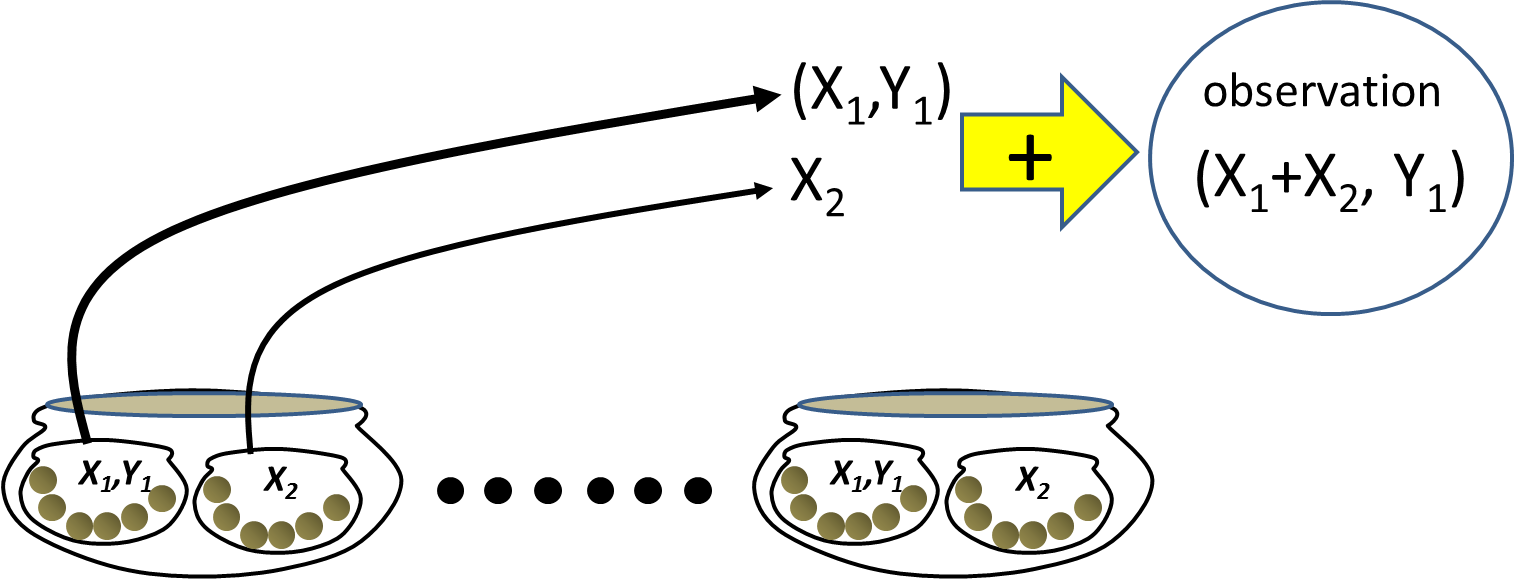
\includegraphics[scale=0.4]{figs/generation.png}
\end{center}

Thus, the final observation is:
$$(X,Y) =  (X_1 + X_2, Y_1)$$
Representing the output random variable as $(x,y)$, the probability that it takes a value $(X,Y)$ is given by $P_{x,y}(X,Y)$.


\begin{enumerate}
    \item Give the expression for $P_{x,y}(X,Y)$ in terms of $P_z(Z)$, $P_{x_1,y_1}(X_1,Y_1|Z)$ and  $P_{x_2}(X_2|Z)$. Please, \ul{submit your expressions with the proper explanation as part of your report}.
    \item You are given a histogram of counts $H(X,Y)$ obtained from a large number of observations.  $H(X,Y)$ represents the number of times  $(X,Y)$ was observed. Give the EM update rules to estimate $P_z(Z)$, $P_{x_1,y_1}(X_1,Y_1|Z)$ and  $P_{x_2}(X_2|Z)$. \ul{Submit your aswer with the proper explanation as part of your report}.

\end{enumerate}
 


\subsection{Application to Deblurring }

In this problem we will try to deblur a picture that has become blurry due to a slight left-to-right shake of the camera. You can find the actual picture in \texttt{hw4materials/problem2}.
\begin{center}
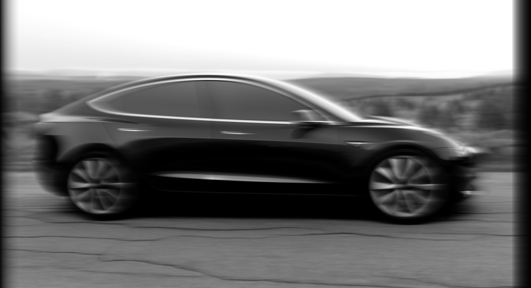
\includegraphics[scale=0.4]{figs/carblurred.png}
\end{center}
We model the picture as a histogram (the value of any pixel at a position $(X,Y)$, which ranges from 0-255, is viewed as the count of ``light elements'' at that position). We model this distribution as a shift-invariant mixture of one component (i.e. one large urn). 
\\
\\
Assuming a very slight 20-pixel strictly-horizontal shake, we model that within the $X_2$ sub-urn $X_2$ can take integer values 0-19 (i.e. 20 wide). The $X_1$ value in the $(X_1,Y_1)$ sub-urn can range from 0 to (width-of-picture - 20). $Y_1$ can take values in the range 0 to (height-of-picture - 1). 
\\
\\
\begin{enumerate}
    \item Write a script that takes as input a histogram $H(X,Y)$ and using the EM algorithm returns $P_{x_2}(X_2)$ and $P_{x_1,y_1}(X_1, Y_1)$. \ul{Submit your code}.
    \item Using the image provided, estimate and plot $P_{x_2}(X_2)$ and $P_{x_1,y_1}(X_1, Y_1)$. You will need the solution to problem 2.1 for this problem. 
    %If the solution to problem 2.1 is incorrect, the solution of this problem will not be considered or given any points.
    \ul{Attach your estimation of $P_{x_1,y_1}(X_1, Y_1)$ as image to your report}.
\end{enumerate}






